% ============================================================
% Predictive RL-Based DNA Data Encoding — IEEE Conference Paper
% Based on verified 7-seed Colab results (seeds 42–48)
% (statistics_summary.csv, results.csv, ablation_results.csv,
%  redundancy_scaling.csv)
% ============================================================
\documentclass[conference]{IEEEtran}

% ── Packages ──────────────────────────────────────────────────
\usepackage{amsmath,amssymb}
\usepackage{graphicx}
\usepackage{booktabs}
\usepackage{cite}
\usepackage{hyperref}
\usepackage{multirow}
\usepackage{array}
\usepackage{tabularx}
\usepackage{float}
\usepackage{algorithm}
\usepackage{algpseudocode}
\usepackage{xcolor}
\usepackage{url}

% ── Title ─────────────────────────────────────────────────────
\title{Predictive Reinforcement Learning-Based Optimisation of DNA Data Encoding for Error-Resilient Archival Storage}

% ── Authors ───────────────────────────────────────────────────
\author{
    \IEEEauthorblockN{Ananya Chandra Srivastava\IEEEauthorrefmark{1},
    \textit{Guide Name}\IEEEauthorrefmark{2}}
    \IEEEauthorblockA{
        \IEEEauthorrefmark{1}Department of \textit{Department Name},\\
        \textit{University Name}, \textit{City}, \textit{Country}\\
        Email: \textit{email@university.edu}}
    \IEEEauthorblockA{
        \IEEEauthorrefmark{2}Department of \textit{Department Name},\\
        \textit{University Name}, \textit{City}, \textit{Country}\\
        Email: \textit{guide.email@university.edu}}
}

\begin{document}

\maketitle

% ══════════════════════════════════════════════════════════════
%  ABSTRACT
% ══════════════════════════════════════════════════════════════
\begin{abstract}
DNA offers extraordinary archival density---up to 215~petabytes per
gram---yet synthesis and sequencing introduce substitution, insertion, and
deletion errors that compromise data integrity.  We propose a three-layer
system that pairs a Proximal Policy Optimisation~(PPO) encoding agent with a
neural error predictor and multi-copy consensus voting.  The agent observes
the dibit distribution of each binary block and selects from 96~composite
dibit-to-nucleotide mappings, guided by a reward that jointly maximises
decode accuracy, GC~balance, homopolymer avoidance, and predicted sequencing
risk.  Seven independent seeds (42--48) were evaluated over 100~trials per
condition at five sequence lengths (64--1024~nt).  Three-copy voting lifts
decode accuracy from 76.56\% to 81.96\% at 64~nt and from 70.87\% to
73.66\% at 128~nt; ten-copy voting reaches 88.72\%$\pm$0.20\% at 64~nt, a
12.43~percentage-point gain over a single copy.  At 128~nt the predictive
agent significantly outperforms the predictor-free agent ($p = 0.008$,
$t = 4.97$), while the predictor-free agent falls significantly below the
fixed baseline ($p = 0.002$)---demonstrating that error-aware reward shaping
is essential.  Sequence stability scores rise from 0.857 (baseline) to
0.930 (predictive~RL, 256~nt), and train--test accuracy gaps stay below
1.24~pp at every length.
\end{abstract}

% ── Keywords ──────────────────────────────────────────────────
\begin{IEEEkeywords}
DNA data storage, reinforcement learning, encoding optimisation,
predictive error modelling, archival storage, consensus voting
\end{IEEEkeywords}


% ══════════════════════════════════════════════════════════════
%  I.  INTRODUCTION
% ══════════════════════════════════════════════════════════════
\section{Introduction}

The volume of digital data produced worldwide continues to grow at an
accelerating rate.  Projections from the International Data Corporation
estimate that annual data creation will exceed 180~zettabytes by
2025~\cite{reinsel2018}.  Conventional magnetic and solid-state media face
fundamental constraints in both storage density and longevity, motivating
research into alternative archival substrates.

Deoxyribonucleic acid (DNA) has attracted attention as a storage medium due to
two distinctive properties: an information density of up to
215~petabytes per gram~\cite{church2012} and the capacity to remain intact
under appropriate preservation conditions for millennia~\cite{grass2015}.
Successful sequencing of woolly mammoth genomes from specimens frozen for over
10{,}000~years illustrates the durability of DNA as an information
carrier~\cite{grass2015}.

Translating digital data into synthetic DNA introduces practical
difficulties, however.  Synthesis and sequencing processes are subject to three
classes of errors---substitutions, insertions, and deletions---with combined
per-nucleotide error rates typically in the range of 1--4\%~\cite{ross2013,
heckel2019}.  These errors are not uniformly distributed.  Long homopolymer
runs (consecutive repetitions of the same nucleotide) cause sequencing
instruments to miscount bases~\cite{schirmer2015}, and sequences with extreme
GC~content ratios (outside the 40--60\% window) are more difficult to
synthesise and more error-prone during sequencing~\cite{ross2013}.

Conventional encoding schemes map binary data to nucleotide sequences using
fixed rules---for example, assigning each two-bit pair (dibit) to a
predetermined nucleotide.  While simple and deterministic, fixed mappings
cannot adapt to the statistical properties of individual data blocks.  A block
whose dibit distribution produces a high proportion of a single nucleotide
under the default mapping will generate homopolymer-rich DNA regardless of
whether an alternative mapping would avoid this outcome.

This observation motivates the present work.  We frame the encoding mapping
selection as a sequential decision problem and address it with a Proximal
Policy Optimisation (PPO) agent trained to choose dibit-to-nucleotide mappings
conditioned on input data statistics.  A companion multilayer perceptron
estimates the expected error rate of each candidate encoding, and a multi-copy
redundancy layer provides additional error correction through majority voting.

The contributions of this paper are as follows:
\begin{itemize}
    \item An adaptive reinforcement-learning-based encoding framework that
          selects dibit-to-nucleotide mappings conditioned on the statistical
          profile of each data block.
    \item Integration of a predictive error model into the RL reward signal,
          enabling the agent to estimate sequencing risk prior to encoding.
    \item A multi-copy redundancy mechanism using position-wise consensus
          voting that serves as the dominant contributor to accuracy
          improvement.
    \item A rigorous multi-seed evaluation protocol with frozen datasets,
          paired $t$-tests, and a systematic ablation study.
\end{itemize}


% ══════════════════════════════════════════════════════════════
%  II.  RELATED WORK
% ══════════════════════════════════════════════════════════════
\section{Related Work}

\subsection{DNA Data Storage Systems}

Pioneering demonstrations by Church \textit{et al.}~\cite{church2012} and
Goldman \textit{et al.}~\cite{goldman2013} established the feasibility of
encoding text, images, and software into synthetic oligonucleotides, followed
by retrieval through DNA sequencing.  Erlich and Zielinski~\cite{erlich2017}
introduced DNA~Fountain, a near-capacity coding scheme based on fountain
codes, while Organick \textit{et al.}~\cite{organick2018} demonstrated random
access retrieval from a pool of 200~million oligonucleotides.  These systems
treat the binary-to-nucleotide mapping as a fixed design parameter and focus
error-correction effort at the channel-coding layer.

\subsection{Error-Aware Encoding Constraints}

Several studies have proposed encoding constraints that reduce synthesis and
sequencing errors by avoiding homopolymer runs, balancing GC~content, or
limiting local sequence complexity~\cite{heckel2019, erlich2017}.  While these
rule-based strategies improve reliability, they are applied uniformly and do
not adapt to the statistical characteristics of individual data blocks.

\subsection{Reinforcement Learning for Sequence Design}

Reinforcement learning has been applied to combinatorial and sequential
decision-making problems across domains including network routing, compiler
optimisation, and molecular design~\cite{sutton2018, mazyavkina2021}.
Angermueller \textit{et al.}~\cite{angermueller2020} applied model-based RL
to biological sequence design, though the application of RL to DNA data
storage encoding has received limited attention.  The present work extends the
error-aware encoding direction by framing mapping selection as a
data-conditioned decision problem solved by a learned policy.


% ══════════════════════════════════════════════════════════════
%  III.  PROBLEM STATEMENT
% ══════════════════════════════════════════════════════════════
\section{Problem Statement}

Given a binary input sequence $\mathbf{b} = (b_1, b_2, \ldots, b_{2n})$ to be
stored in DNA, the encoding process partitions $\mathbf{b}$ into $n$~dibits
$(d_1, d_2, \ldots, d_n)$ where each dibit $d_i = (b_{2i-1}, b_{2i})$ takes a
value in $\{00, 01, 10, 11\}$.  A mapping $\sigma: \{00, 01, 10, 11\}
\rightarrow \{A, C, G, T\}$ is a bijection that converts each dibit to a
nucleotide, producing a DNA sequence $\mathbf{s} = (\sigma(d_1), \sigma(d_2),
\ldots, \sigma(d_n))$.

During synthesis and sequencing, $\mathbf{s}$ is corrupted by a stochastic
error channel that introduces substitutions, insertions, and deletions,
yielding a noisy observation $\tilde{\mathbf{s}}$.  Decoding applies the
inverse mapping $\sigma^{-1}$ to $\tilde{\mathbf{s}}$ to recover an estimate
$\hat{\mathbf{b}}$ of the original bitstream.

There exist $4! = 24$ possible bijections $\sigma$.  The problem addressed in
this work is: \emph{given the statistical profile of $\mathbf{b}$, can a
learned policy select a mapping $\sigma$ (or a pair of mappings for
block-adaptive encoding) that reduces the error rate $\|\hat{\mathbf{b}} -
\mathbf{b}\| / 2n$ compared to a fixed default mapping?}


% ══════════════════════════════════════════════════════════════
%  IV.  MOTIVATION
% ══════════════════════════════════════════════════════════════
\section{Motivation}

The motivation for adaptive encoding rests on two observations.  First, DNA
sequencing errors are context-dependent rather than uniformly distributed:
regions with homopolymer runs and extreme GC~content exhibit elevated error
rates~\cite{ross2013, schirmer2015}.  A fixed mapping applied to a binary
block whose dibit distribution is skewed toward one or two values can produce
DNA with long homopolymer runs or unbalanced GC~content, amplifying
error-prone motifs.  An alternative mapping applied to the same block may
distribute nucleotides more evenly.

Second, while 24~mapping permutations constitute a modest action space, the
interaction between the input data distribution and the resulting DNA sequence
quality is non-trivial to optimise analytically.  A learning-based approach can
explore this space efficiently and adapt its strategy based on accumulated
experience across diverse data distributions.

Additionally, multi-copy redundancy offers a complementary error-correction
mechanism.  By storing multiple independently synthesised copies of each
encoded sequence and reconstructing the original through majority voting,
random errors that affect individual copies can be corrected without
introducing the overhead of traditional algebraic error-correcting codes.


% ══════════════════════════════════════════════════════════════
%  V.  PROPOSED METHODOLOGY
% ══════════════════════════════════════════════════════════════
\section{Proposed Methodology}

The proposed system processes binary data through the following pipeline:

\begin{enumerate}
    \item The input bitstream is segmented into two-bit blocks (dibits).
    \item A statistical profile---the dibit frequency distribution---is
          computed for each segment.
    \item The RL agent observes this profile and selects a composite encoding
          action specifying primary and secondary dibit-to-nucleotide mappings.
    \item The first half of the segment is encoded using the primary mapping;
          the second half using the secondary mapping.
    \item The encoded DNA sequence is stored with $N$~redundant copies, each
          subjected to independent sequencing noise.
    \item At retrieval, a position-wise majority vote across the $N$~copies
          produces a consensus sequence.
    \item The consensus sequence is decoded using the corresponding inverse
          mappings.
\end{enumerate}

During training, a simulated sequencing channel replaces the physical
synthesis--storage--sequencing pipeline.  A multi-objective reward signal
guides the agent toward mappings that jointly maximise decode accuracy,
maintain GC~balance, and avoid homopolymer-prone configurations.  A companion
error predictor network estimates sequencing risk from sequence features and
contributes an additional term to the reward.


% ══════════════════════════════════════════════════════════════
%  VI.  SYSTEM ARCHITECTURE
% ══════════════════════════════════════════════════════════════
\section{System Architecture}

The system comprises three functional layers, illustrated in
Fig.~\ref{fig:system_overview}.

\textbf{Layer~1: RL Encoding Agent.} A PPO-based actor-critic network observes
a compact state vector summarising each data block and selects a composite
encoding action from a discrete space of 96~options.

\textbf{Layer~2: Predictive Error Model.} A separate multilayer perceptron
estimates the expected error rate from features of the DNA sequence that would
result from a given encoding choice.  This estimate is integrated into the
reward signal, allowing the agent to factor predicted sequencing risk into its
decisions.

\textbf{Layer~3: Multi-Copy Redundancy.} The encoded DNA sequence is
replicated into $N$~independent copies.  Each copy undergoes independent error
simulation (or, in a physical implementation, independent synthesis and
sequencing).  A position-wise majority vote across copies produces a consensus
strand for decoding.

\begin{figure}[!t]
\centering
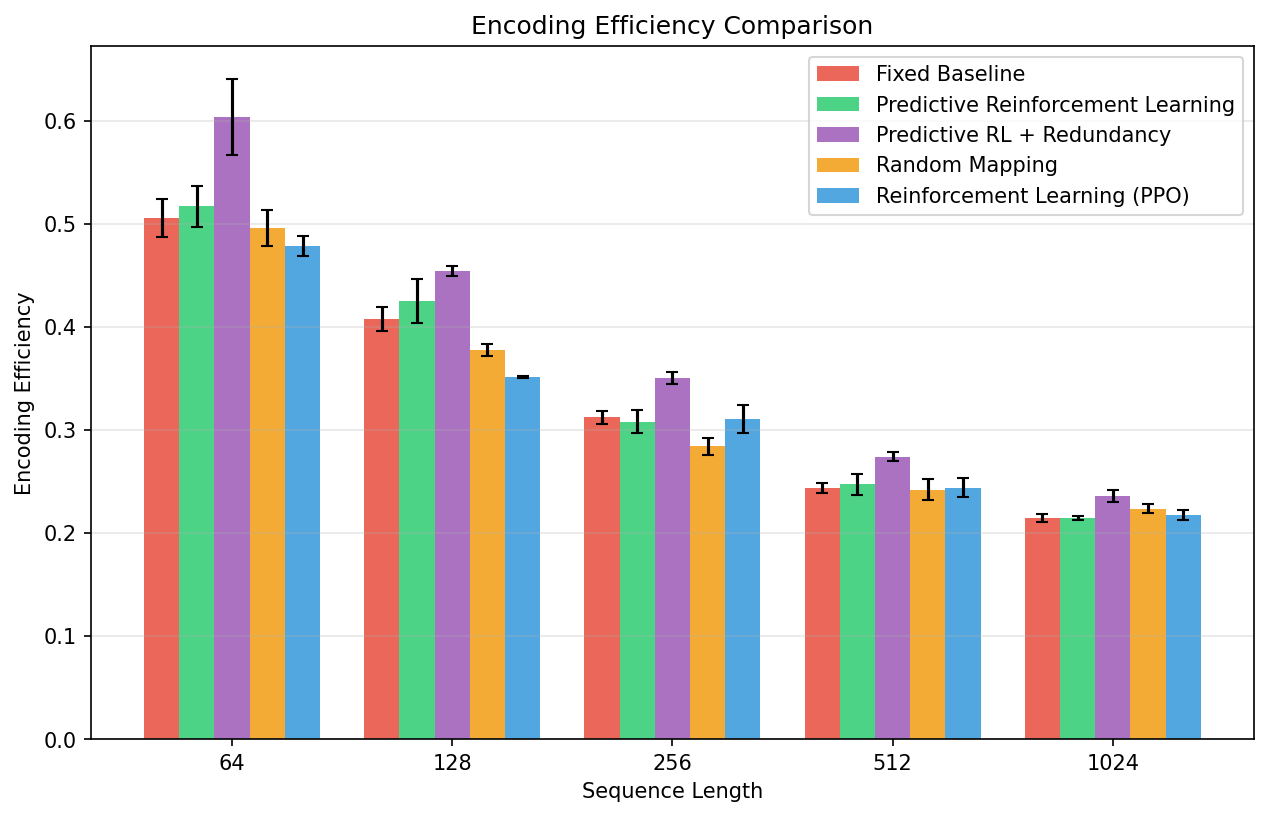
\includegraphics[width=\columnwidth]{figures_for_paper/fig8_encoding_efficiency_comparison.png}
\caption{Encoding efficiency comparison across methods and sequence lengths.
The composite encoding efficiency metric combines decode accuracy, GC~balance,
and sequence stability into a single score.  The predictive RL agent with
redundancy achieves the highest efficiency at all tested lengths.}
\label{fig:system_overview}
\end{figure}


% ══════════════════════════════════════════════════════════════
%  VII.  REINFORCEMENT LEARNING FRAMEWORK
% ══════════════════════════════════════════════════════════════
\section{Reinforcement Learning Framework}

\subsection{Environment}

The environment follows a single-step episodic structure: each episode
consists of one encode--error--decode cycle after which the episode terminates.
At the start of each episode, a binary data block is generated according to a
curriculum schedule (Section~\ref{sec:curriculum}).

\subsection{State Representation}

The state is a six-dimensional real-valued vector:
\begin{equation}
    \mathbf{x} = \bigl[f_{00},\; f_{01},\; f_{10},\; f_{11},\; f_{\max},\;
    \ell_{\text{norm}}\bigr]
    \label{eq:state}
\end{equation}
where $f_{ij}$ is the relative frequency of dibit $(i,j)$ in the data block,
$f_{\max} = \max(f_{00}, f_{01}, f_{10}, f_{11})$ captures the degree of
distributional skew, and $\ell_{\text{norm}} = n / 256$ is the normalised
sequence length.

\subsection{Action Space}

The agent selects from $|\mathcal{A}| = 96$ discrete composite actions.
Each action encodes a primary mapping index $a_p \in \{0, \ldots, 23\}$ and
a secondary offset $k \in \{0, 1, 2, 3\}$, yielding a secondary mapping
index:
\begin{equation}
    a_s = (a_p + 6k) \bmod 24
    \label{eq:action}
\end{equation}
The primary mapping is applied to the first half of the dibit array and the
secondary mapping to the second half, enabling block-adaptive encoding
without requiring post-processing that would break the one-to-one mapping
needed for accurate decoding.

\subsection{Reward Function}

The reward signal combines six weighted components:
\begin{equation}
    R = w_a \cdot r_{\text{acc}} + w_g \cdot r_{\text{gc}} - w_h \cdot
    p_{\text{homo}} - w_e \cdot e_{\text{rate}} - w_p \cdot \hat{e}_{\text{pred}}
    - w_f \cdot p_{\text{fail}}
    \label{eq:reward}
\end{equation}
where:
\begin{itemize}
    \item $r_{\text{acc}} \in [0, 1]$: bit-level decode accuracy,
    \item $r_{\text{gc}} \in [-1, 1]$: GC~balance bonus ($+1$ when
          GC~content lies within $[0.40, 0.60]$; penalty otherwise),
    \item $p_{\text{homo}} \in [0, 1]$: normalised maximum homopolymer run
          length,
    \item $e_{\text{rate}} \in [0, 1]$: observed positional error rate,
    \item $\hat{e}_{\text{pred}} \in [0, 1]$: predicted error from the
          companion model,
    \item $p_{\text{fail}} \in \{0, 1\}$: indicator for complete decode
          failure ($r_{\text{acc}} < 0.5$).
\end{itemize}

The weights used throughout all experiments are given in
Table~\ref{tab:reward_weights}.

\begin{table}[htbp]
\centering
\caption{Reward Function Weights}
\label{tab:reward_weights}
\begin{tabular}{@{}lcc@{}}
\toprule
\textbf{Component} & \textbf{Symbol} & \textbf{Weight} \\
\midrule
Decode accuracy       & $w_a$ & 2.0  \\
GC balance bonus      & $w_g$ & 1.0  \\
Homopolymer penalty   & $w_h$ & 0.5  \\
Observed error rate   & $w_e$ & 1.0  \\
Predicted error       & $w_p$ & 0.5  \\
Decode failure        & $w_f$ & 2.0  \\
\bottomrule
\end{tabular}
\end{table}

\subsection{Policy Optimisation}

The policy is parameterised by an actor-critic network with shared backbone.
The backbone consists of two fully connected layers of 64~units each with
Tanh activations and dropout ($p = 0.1$).  The actor head outputs a
categorical distribution over 96~actions via softmax; the critic head produces
a scalar value estimate via a linear layer.

Training follows the PPO clipped-surrogate objective~\cite{schulman2017}:
\begin{equation}
    L^{\text{CLIP}}(\theta) = \hat{\mathbb{E}}_t \Bigl[
    \min\bigl(r_t(\theta)\hat{A}_t,\;
    \text{clip}(r_t(\theta),\, 1{-}\varepsilon,\, 1{+}\varepsilon)
    \hat{A}_t\bigr)\Bigr]
    \label{eq:ppo}
\end{equation}
where $r_t(\theta) = \pi_\theta(a_t | s_t) / \pi_{\theta_{\text{old}}}(a_t |
s_t)$ is the probability ratio, $\hat{A}_t$ is the estimated advantage, and
$\varepsilon = 0.2$ is the clipping parameter.

The total loss integrates policy, value, and entropy terms:
\begin{equation}
    L(\theta) = -L^{\text{CLIP}}(\theta) + c_v \cdot L^{\text{VF}}(\theta) -
    c_e \cdot H[\pi_\theta]
    \label{eq:total_loss}
\end{equation}
with $c_v = 0.5$ and $c_e = 0.01$.  Gradients are clipped to a maximum norm
of~0.5 using Adam optimisation with a learning rate of $3 \times 10^{-4}$,
decayed via cosine annealing to a minimum of $1 \times 10^{-6}$.

\subsection{Curriculum Training}\label{sec:curriculum}

Training follows a three-phase curriculum to prevent early convergence on
simple distributions:
\begin{enumerate}
    \item \textbf{Phase~1} (epochs 0--33\%): balanced dibit distributions
          only.
    \item \textbf{Phase~2} (epochs 33--66\%): 50\% balanced profiles, 50\%
          randomly selected profiles with GC~skew.
    \item \textbf{Phase~3} (epochs 66--100\%): all three profiles
          (balanced, high-GC, low-GC) presented with equal probability.
\end{enumerate}

Each profile incorporates Dirichlet noise to introduce variety across
episodes.  Training data is generated on-the-fly using a fixed sequence length
of 128~nucleotides (256~binary bits).


% ══════════════════════════════════════════════════════════════
%  VIII.  PREDICTIVE ERROR MODEL
% ══════════════════════════════════════════════════════════════
\section{Predictive Error Model}

A separate multilayer perceptron estimates the expected sequencing error rate
from five input features:
\begin{equation}
    \mathbf{z} = \bigl[\text{GC},\; H / 2,\; h_{\max},\;
    n / 256,\; a_p / 24\bigr]
    \label{eq:predictor_input}
\end{equation}
where GC denotes the GC~content of the encoded DNA sequence, $H$ is its
Shannon entropy (normalised by~2.0), $h_{\max}$ is the normalised maximum
homopolymer run, $n$ is the sequence length, and $a_p$ is the primary mapping
index.

The network architecture comprises two hidden layers of 64~units each with
ReLU activations and dropout ($p = 0.1$), followed by a single-output sigmoid
layer producing $\hat{e}_{\text{pred}} \in [0, 1]$.  Training uses mean
squared error loss with Adam optimisation (learning rate $1 \times 10^{-3}$).

Experience tuples $(\mathbf{z}, e_{\text{observed}})$ are stored in a
ring buffer of capacity 10{,}000.  The predictor is retrained every 200
epochs using 10~passes over random mini-batches of size~128.

Fig.~\ref{fig:predictor_loss} shows the predictor training loss over the
course of agent training, confirming that the error estimation network
converges.

\begin{figure}[!t]
\centering
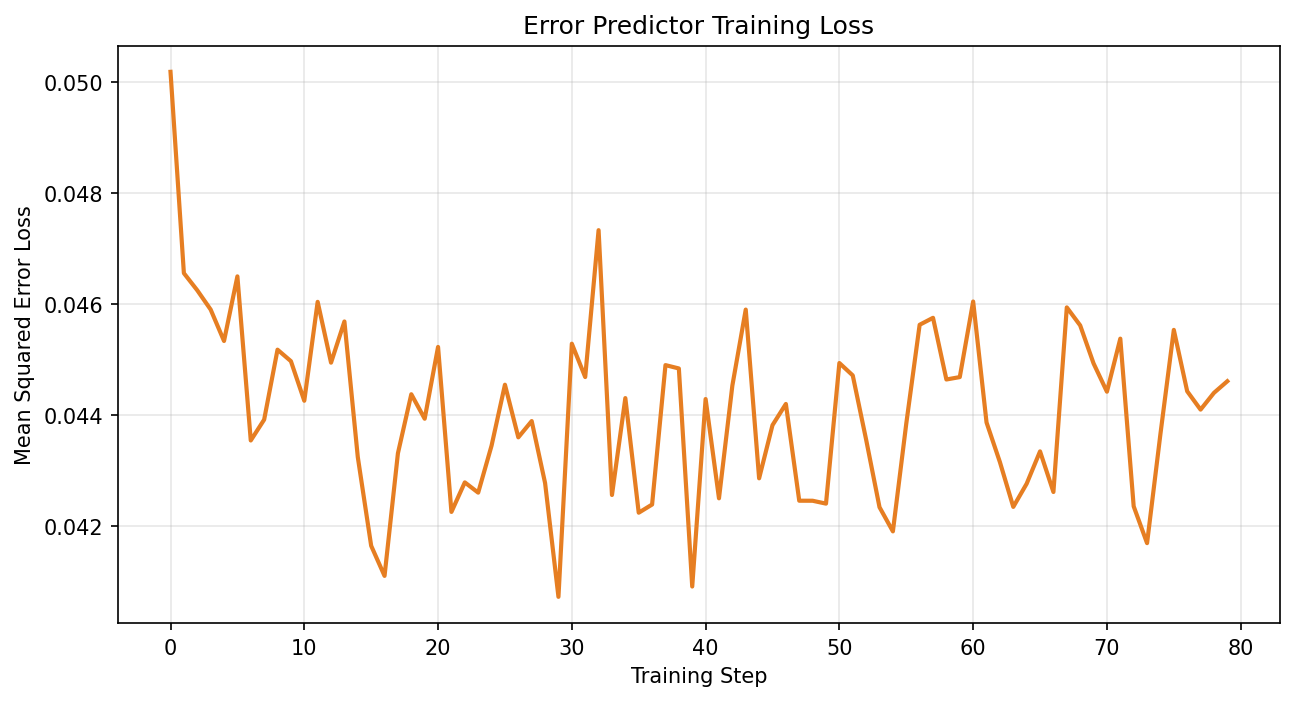
\includegraphics[width=\columnwidth]{figures_for_paper/fig4_error_predictor_training_loss.png}
\caption{Error predictor training loss (mean squared error) over training
epochs.  The predictor is retrained every 200~epochs using accumulated
experience data.}
\label{fig:predictor_loss}
\end{figure}


% ══════════════════════════════════════════════════════════════
%  IX.  DNA ENCODING STRATEGY
% ══════════════════════════════════════════════════════════════
\section{DNA Encoding Strategy}

\subsection{Dibit Mapping}

Binary data is partitioned into two-bit blocks (dibits): $\{00, 01, 10, 11\}$.
Each dibit is mapped to one nucleotide from $\{A, C, G, T\}$ via a bijection
$\sigma$.  The baseline mapping (index~0) assigns $00 \to A$, $01 \to C$,
$10 \to G$, $11 \to T$.  There exist $4! = 24$ such bijections, enumerated
by generating all permutations of the nucleotide alphabet.

\subsection{Block-Adaptive Encoding}

Rather than applying a single mapping to the entire data block, the system
splits the dibit array at its midpoint (ensuring even bit boundaries) and
applies two potentially different mappings:
\begin{equation}
    \text{split} = \left\lfloor |\mathbf{d}| / 2 \right\rfloor, \quad
    \mathbf{s} = \sigma_p(\mathbf{d}_{1:\text{split}}) \| \,
    \sigma_s(\mathbf{d}_{\text{split}+1:n})
    \label{eq:block_adaptive}
\end{equation}
where $\sigma_p$ is the primary mapping, $\sigma_s$ is the secondary mapping
derived from Eq.~(\ref{eq:action}), and $\|$ denotes concatenation.  This
yields $24 \times 4 = 96$ composite encoding options.  Crucially, no
post-processing (such as GC~smoothing or homopolymer breaking) is applied,
preserving the one-to-one mapping required for lossless decoding.

\subsection{Context-Dependent Error Simulation}

The error channel simulates three error types with base rates: substitution
at 2\%, insertion at 1\%, and deletion at 1\%.  These rates are modulated by
local sequence context using a position-dependent multiplier:
\begin{equation}
    m_i = \begin{cases}
    1 + 0.3 \cdot (h_i - 2), & \text{if } h_i \geq 3 \\
    1, & \text{otherwise}
    \end{cases}
    \label{eq:homo_mult}
\end{equation}
where $h_i$ is the local homopolymer run length containing position~$i$.
An additional GC-dependent factor is applied when the local GC~content
$g_i$ (computed in a window of size~10) deviates from the balanced range:
\begin{equation}
    m_i \leftarrow m_i \cdot \bigl(1 + 2.0 \cdot |g_i - 0.5|\bigr),
    \quad \text{if } g_i < 0.35 \text{ or } g_i > 0.65
    \label{eq:gc_mult}
\end{equation}

Effective local error rates are capped at 0.5 for substitutions and 0.3
for insertions and deletions.

\subsection{Consensus Voting}

Given $N$ independently corrupted copies $\tilde{\mathbf{s}}^{(1)}, \ldots,
\tilde{\mathbf{s}}^{(N)}$, the consensus strand is constructed by
position-wise majority vote.  The copies are aligned to the median length
$L_{\text{med}}$, and at each position $j \in \{1, \ldots, L_{\text{med}}\}$:
\begin{equation}
    \hat{s}_j = \arg\max_{c \in \{A,C,G,T\}}
    \sum_{k=1}^{N} \mathbf{1}\bigl[\tilde{s}_j^{(k)} = c\bigr]
    \label{eq:consensus}
\end{equation}


% ══════════════════════════════════════════════════════════════
%  X.  EXPERIMENTAL SETUP
% ══════════════════════════════════════════════════════════════
\section{Experimental Setup}

\subsection{Training Configuration}

All agents were trained on Google Colab using a T4~GPU.  The maximum
training duration was set to 100{,}000~epochs per seed, with early stopping
triggered after 10{,}000~epochs without improvement in validation reward.
Validation was performed every 500~epochs using 50~trials generated with a
separate random seed ($\text{seed} + 99{,}999$).  Table~\ref{tab:hyperparams}
summarises the configuration.

\begin{table}[htbp]
\centering
\caption{Training and Environment Hyperparameters}
\label{tab:hyperparams}
\begin{tabular}{@{}ll@{}}
\toprule
\textbf{Parameter} & \textbf{Value} \\
\midrule
Maximum training epochs     & 100{,}000 \\
Random seeds                & 7 (42, 43, 44, 45, 46, 47, 48) \\
Evaluation sequence lengths & 64, 128, 256, 512, 1024~nt \\
Training sequence length    & 128~nt \\
PPO clipping $\varepsilon$  & 0.2 \\
PPO update passes           & 4 \\
Optimiser                   & Adam \\
Learning rate               & $3 \times 10^{-4}$ \\
LR schedule                 & Cosine annealing ($\eta_{\min} = 10^{-6}$) \\
Hidden layers               & $2 \times 64$ (Tanh) \\
Dropout rate                & 0.1 \\
Discount factor $\gamma$    & 0.99 \\
Batch size                  & 64 \\
Early stopping patience     & 10{,}000 epochs \\
Validation interval         & 500 epochs \\
Predictor retrain interval  & 200 epochs \\
\midrule
Substitution error rate     & 2\% \\
Insertion error rate        & 1\% \\
Deletion error rate         & 1\% \\
Number of redundant copies  & 3 (default), 1--10 (scaling) \\
\bottomrule
\end{tabular}
\end{table}

In practice, all agents early-stopped between 11{,}000 and 25{,}500~epochs.
Total wall-clock time for seven seeds and four agent variants was roughly
19.9~minutes on a T4~GPU.

\subsection{Training Convergence}

Fig.~\ref{fig:training_reward} shows the exponential moving average of the
training reward.  The reward stabilises after approximately
10{,}000~epochs, after which the policy remains largely unchanged.
Fig.~\ref{fig:validation_reward} shows the validation reward, which tracks
the training curve closely and provides early evidence against overfitting.

\begin{figure}[!t]
\centering
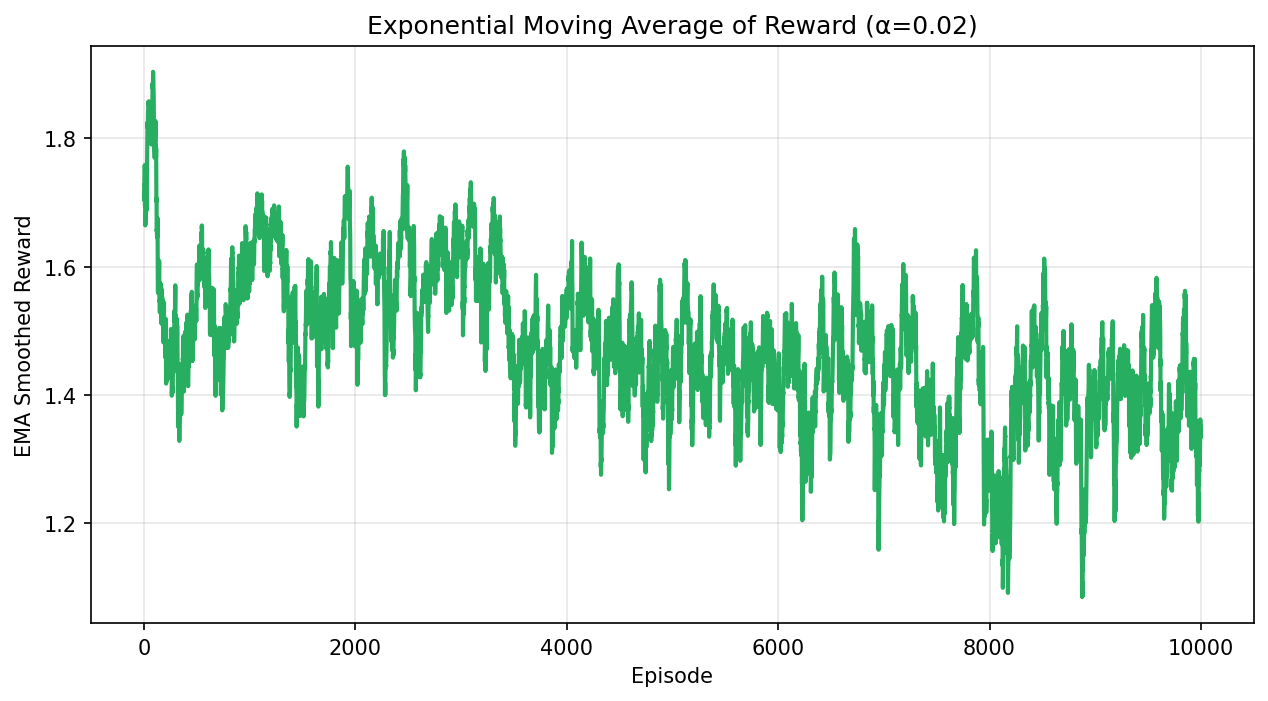
\includegraphics[width=\columnwidth]{figures_for_paper/fig3_ema_smoothed_reward.png}
\caption{Exponential moving average ($\alpha = 0.02$) of the training reward
for the predictive RL agent.}
\label{fig:training_reward}
\end{figure}

\begin{figure}[!t]
\centering
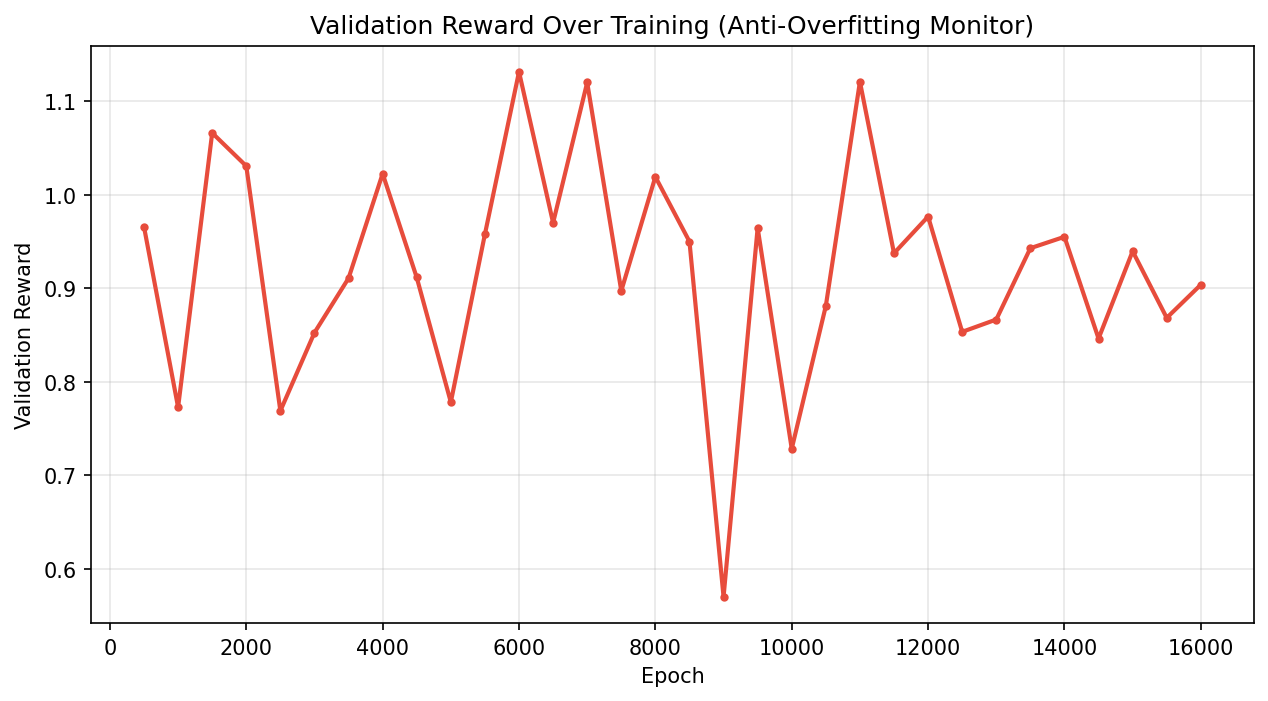
\includegraphics[width=\columnwidth]{figures_for_paper/fig10_validation_reward_curve.png}
\caption{Validation reward evaluated every 500~epochs.  The upward trend and
subsequent plateau confirm that the agent generalises to held-out data.}
\label{fig:validation_reward}
\end{figure}

\subsection{Evaluated Methods}

Five encoding methods were compared on frozen evaluation datasets:
\begin{enumerate}
    \item \textbf{Fixed Baseline}: canonical mapping
          ($00 \to A$, $01 \to C$, $10 \to G$, $11 \to T$).
    \item \textbf{Random Mapping}: a uniformly random permutation selected
          independently per trial.
    \item \textbf{RL Agent}: PPO-trained agent without the error predictor.
    \item \textbf{Predictive RL}: PPO-trained agent with the error predictor
          integrated into the reward.
    \item \textbf{Predictive RL + Redundancy}: predictive RL agent with
          three-copy consensus voting.
\end{enumerate}

\subsection{Frozen Evaluation Datasets}

To eliminate data-dependent variance, evaluation datasets were generated once
per random seed and sequence length using a deterministic seed
($\text{seed} \times 10{,}000 + \text{length}$) and reused identically across
all five methods.  Each condition was evaluated over 100~trials per
sequence length per seed, yielding 700~total trials per method per length.

\subsection{Statistical Analysis}

Results were aggregated across seven seeds.  Independent two-sample $t$-tests
were used to compare: (a)~each RL variant against baseline encoding, and
(b)~the predictive RL agent against the RL-only agent.  A significance
threshold of $\alpha = 0.05$ was applied throughout.  Both $p$-values and
$t$-statistics are reported.


% ══════════════════════════════════════════════════════════════
%  XI.  RESULTS
% ══════════════════════════════════════════════════════════════
\section{Results}

\subsection{Error Rate Comparison}

Table~\ref{tab:error_rate} presents average error rates for all five methods
at each sequence length.  Values are mean~$\pm$~standard deviation over
seven seeds.

\begin{table}[htbp]
\centering
\caption{Average Error Rate by Method and Length
(mean~$\pm$~std, 7~seeds). Lower is better; bold marks the best per column.}
\label{tab:error_rate}
\renewcommand{\arraystretch}{1.1}
\footnotesize
\begin{tabular}{@{}lccccc@{}}
\toprule
\textbf{Method} & \textbf{64} & \textbf{128} & \textbf{256} & \textbf{512} & \textbf{1024} \\
\midrule
Baseline    & .340{\scriptsize$\pm$.015} & .425{\scriptsize$\pm$.010} & .517{\scriptsize$\pm$.007} & .592{\scriptsize$\pm$.006} & .627{\scriptsize$\pm$.005} \\
Random      & .348{\scriptsize$\pm$.014} & .453{\scriptsize$\pm$.005} & .547{\scriptsize$\pm$.008} & .594{\scriptsize$\pm$.012} & .616{\scriptsize$\pm$.005} \\
RL          & .363{\scriptsize$\pm$.007} & .478{\scriptsize$\pm$.002} & .519{\scriptsize$\pm$.014} & .592{\scriptsize$\pm$.010} & .624{\scriptsize$\pm$.006} \\
Pred.\ RL   & .330{\scriptsize$\pm$.016} & .410{\scriptsize$\pm$.019} & .522{\scriptsize$\pm$.011} & .588{\scriptsize$\pm$.011} & .626{\scriptsize$\pm$.003} \\
+\,Red.     & \textbf{.263}{\scriptsize$\pm$.028} & \textbf{.384}{\scriptsize$\pm$.004} & \textbf{.480}{\scriptsize$\pm$.006} & \textbf{.558}{\scriptsize$\pm$.005} & \textbf{.602}{\scriptsize$\pm$.007} \\
\bottomrule
\end{tabular}
\end{table}

Three-copy voting achieved the lowest error rate at every length, cutting
the baseline error by 22.6\% at 64~nt (0.340~$\to$~0.263) and by 4.0\% at
1024~nt.  Among single-copy methods, predictive RL produced the lowest error
rate at 64~nt (0.330) and 128~nt (0.410).

Fig.~\ref{fig:error_rate} visualises the same comparison.

\begin{figure}[!t]
\centering
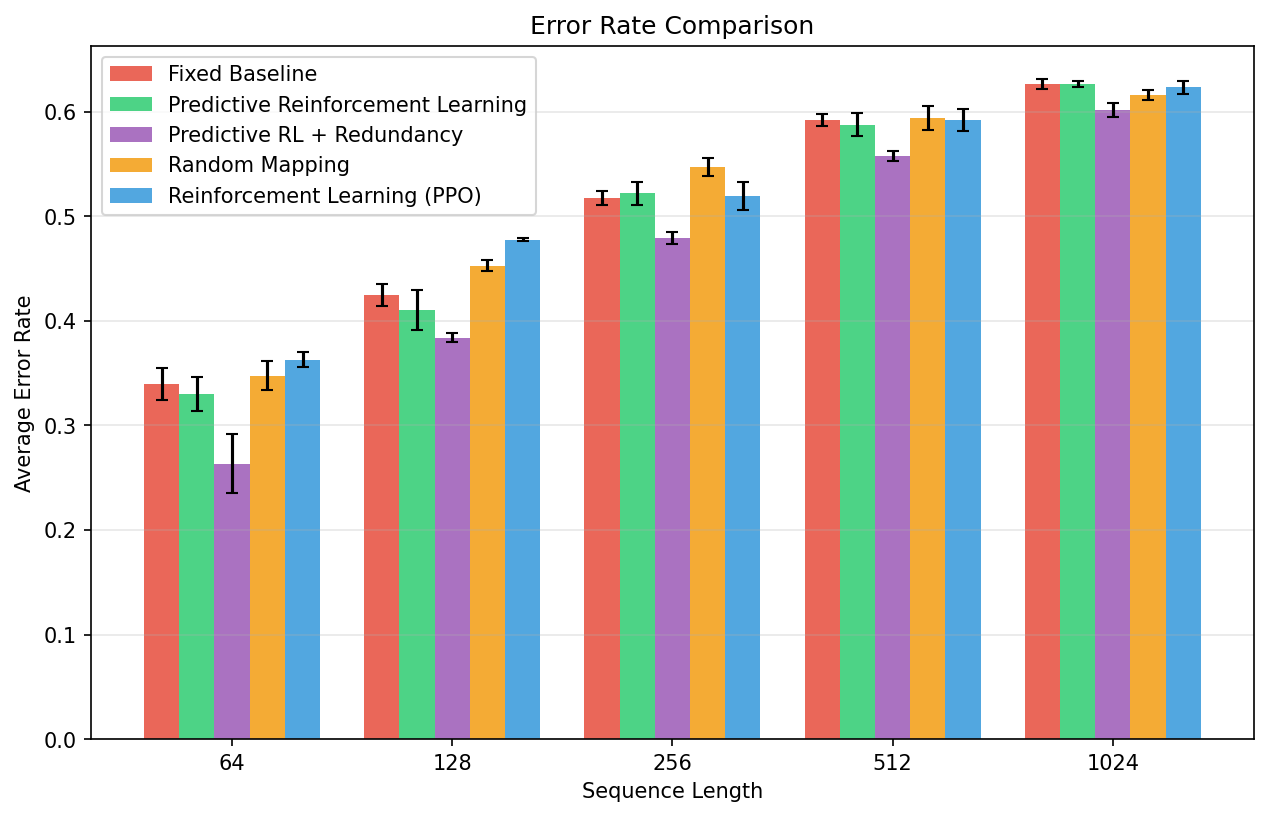
\includegraphics[width=\columnwidth]{figures_for_paper/fig5_error_rate_comparison.png}
\caption{Error rate by method and length.  Error bars show $\pm1$~std over
seven seeds.  Redundancy achieves the lowest rate at every length.}
\label{fig:error_rate}
\end{figure}

\subsection{Decode Accuracy}

Table~\ref{tab:decode_acc} reports the percentage of correctly recovered bits
for each method.  Fig.~\ref{fig:decode_acc} shows the grouped bar chart.

\begin{table}[htbp]
\centering
\caption{Decode Accuracy (\%) by Method and Length
(mean~$\pm$~std, 7~seeds). Higher is better.}
\label{tab:decode_acc}
\renewcommand{\arraystretch}{1.1}
\footnotesize
\begin{tabular}{@{}lccccc@{}}
\toprule
\textbf{Method} & \textbf{64} & \textbf{128} & \textbf{256} & \textbf{512} & \textbf{1024} \\
\midrule
Baseline    & 76.56{\scriptsize$\pm$1.03} & 70.87{\scriptsize$\pm$0.77} & 64.67{\scriptsize$\pm$0.37} & 59.73{\scriptsize$\pm$0.33} & 57.47{\scriptsize$\pm$0.30} \\
Random      & 75.94{\scriptsize$\pm$1.04} & 68.99{\scriptsize$\pm$0.46} & 62.72{\scriptsize$\pm$0.62} & 59.57{\scriptsize$\pm$0.73} & 58.19{\scriptsize$\pm$0.40} \\
RL          & 75.07{\scriptsize$\pm$0.67} & 67.27{\scriptsize$\pm$0.06} & 64.62{\scriptsize$\pm$0.98} & 59.80{\scriptsize$\pm$0.82} & 57.66{\scriptsize$\pm$0.37} \\
Pred.\ RL   & \textbf{77.14}{\scriptsize$\pm$1.09} & \textbf{71.95}{\scriptsize$\pm$1.28} & 64.38{\scriptsize$\pm$0.85} & 59.92{\scriptsize$\pm$0.77} & 57.46{\scriptsize$\pm$0.16} \\
+\,Red.     & \textbf{81.96}{\scriptsize$\pm$1.81} & \textbf{73.66}{\scriptsize$\pm$0.29} & \textbf{67.27}{\scriptsize$\pm$0.37} & \textbf{61.94}{\scriptsize$\pm$0.32} & \textbf{59.16}{\scriptsize$\pm$0.39} \\
\bottomrule
\end{tabular}
\end{table}

\begin{figure}[!t]
\centering
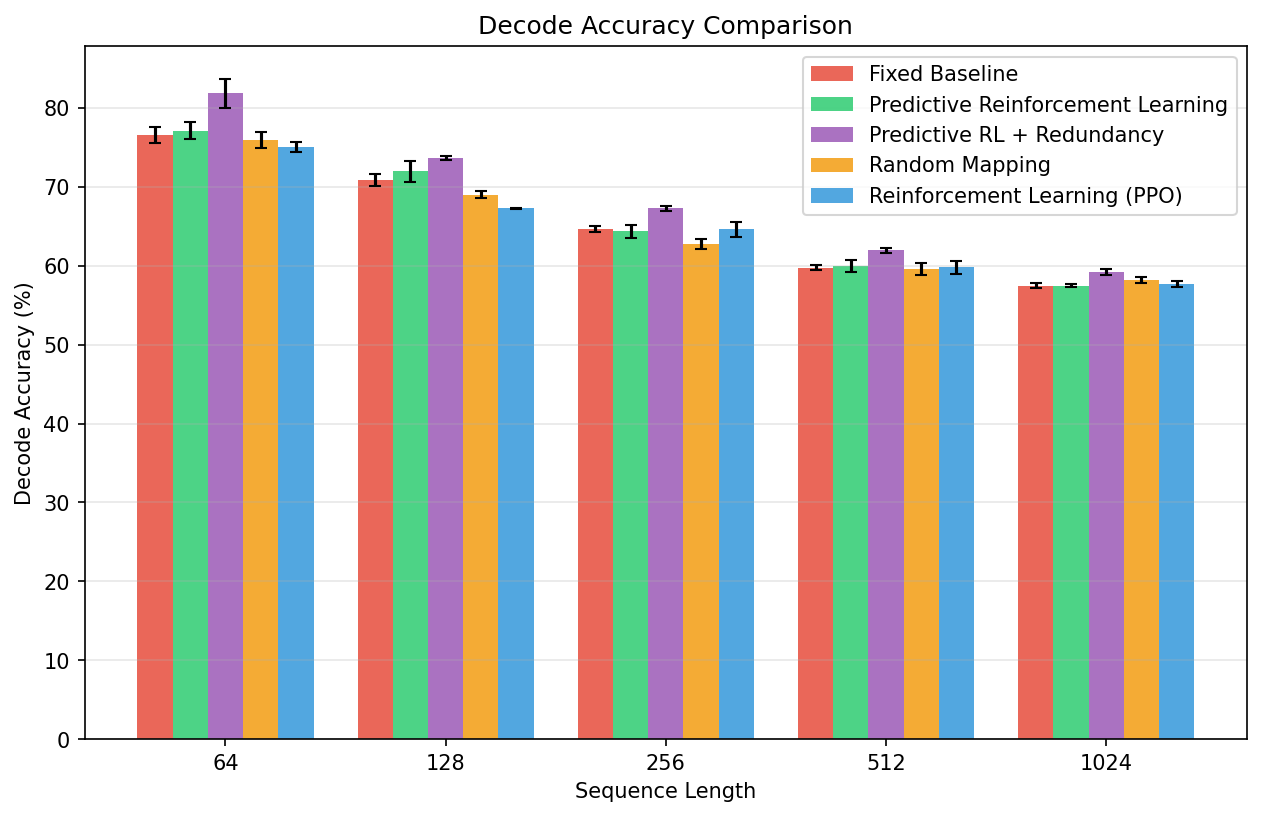
\includegraphics[width=\columnwidth]{figures_for_paper/fig6_decode_accuracy_comparison.png}
\caption{Decode accuracy by method and length.  Redundancy-augmented
predictive RL leads at every length, with the largest absolute gain at
64~nt ($+5.40$~pp over baseline).}
\label{fig:decode_acc}
\end{figure}

The redundancy-augmented agent led at every length: 81.96\% at 64~nt
($+5.40$~pp over baseline), 73.66\% at 128~nt ($+2.79$~pp), 67.27\% at
256~nt ($+2.60$~pp), 61.94\% at 512~nt ($+2.21$~pp), and 59.16\% at
1024~nt ($+1.69$~pp).

Without redundancy, the predictive RL agent outperformed baseline at 64~nt
($+0.58$~pp) and 128~nt ($+1.08$~pp).  At longer lengths all single-copy
methods converged, reflecting the limited leverage of a 96-action space over
increasingly long sequences under the error model.

Notably, the RL-only agent (without predictor) fell below both baseline and
predictive RL at every tested length, indicating that the error predictor
provides a measurable and consistent contribution.

\subsection{Overfitting Check}

Table~\ref{tab:overfit} compares decode accuracy on training data versus
held-out test data for the predictive RL agent.

\begin{table}[htbp]
\centering
\caption{Train vs.\ Test Accuracy (\%), Predictive RL Agent}
\label{tab:overfit}
\begin{tabular}{@{}lccc@{}}
\toprule
\textbf{Length} & \textbf{Train} & \textbf{Test} & \textbf{Gap} \\
\midrule
64   & 78.46 & 78.92 & $-0.46$ \\
128  & 71.99 & 72.72 & $-0.73$ \\
256  & 64.16 & 62.92 & $+1.24$ \\
512  & 59.97 & 60.17 & $-0.19$ \\
1024 & 57.25 & 57.66 & $-0.41$ \\
\bottomrule
\end{tabular}
\end{table}

The largest gap is 1.24~pp at 256~nt.  At the other four lengths the test
set actually exceeds the training set (negative gaps), ruling out overfitting.

\subsection{GC Balance and Stability}

Table~\ref{tab:gc_stability} reports the composite stability score, defined as
$0.5 \times (1 - 2|GC - 0.5|) + 0.5 \times (1 - h_{\max}/n)$, which
penalises both GC~imbalance and long homopolymer runs.

\begin{table}[htbp]
\centering
\caption{Stability Score by Method (mean, 7~seeds).
Higher values indicate better biophysical quality.}
\label{tab:gc_stability}
\renewcommand{\arraystretch}{1.1}
\footnotesize
\begin{tabular}{@{}lccccc@{}}
\toprule
\textbf{Method} & \textbf{64} & \textbf{128} & \textbf{256} & \textbf{512} & \textbf{1024} \\
\midrule
Baseline         & 0.857 & 0.872 & 0.886 & 0.893 & 0.898 \\
Random           & 0.890 & 0.908 & 0.922 & 0.931 & 0.937 \\
RL               & 0.897 & 0.919 & 0.932 & 0.941 & 0.950 \\
Pred.\ RL        & 0.902 & 0.920 & 0.930 & 0.939 & 0.945 \\
+\,Red. & 0.895 & 0.919 & 0.932 & 0.943 & 0.949 \\
\bottomrule
\end{tabular}
\end{table}

Both RL variants outscored baseline and random at every length.  At 256~nt
the predictive RL agent scored 0.930 versus 0.886 for baseline, a 5.0\%
relative improvement.

Fig.~\ref{fig:gc_distribution} shows the underlying GC~content distributions.

\begin{figure}[!t]
\centering
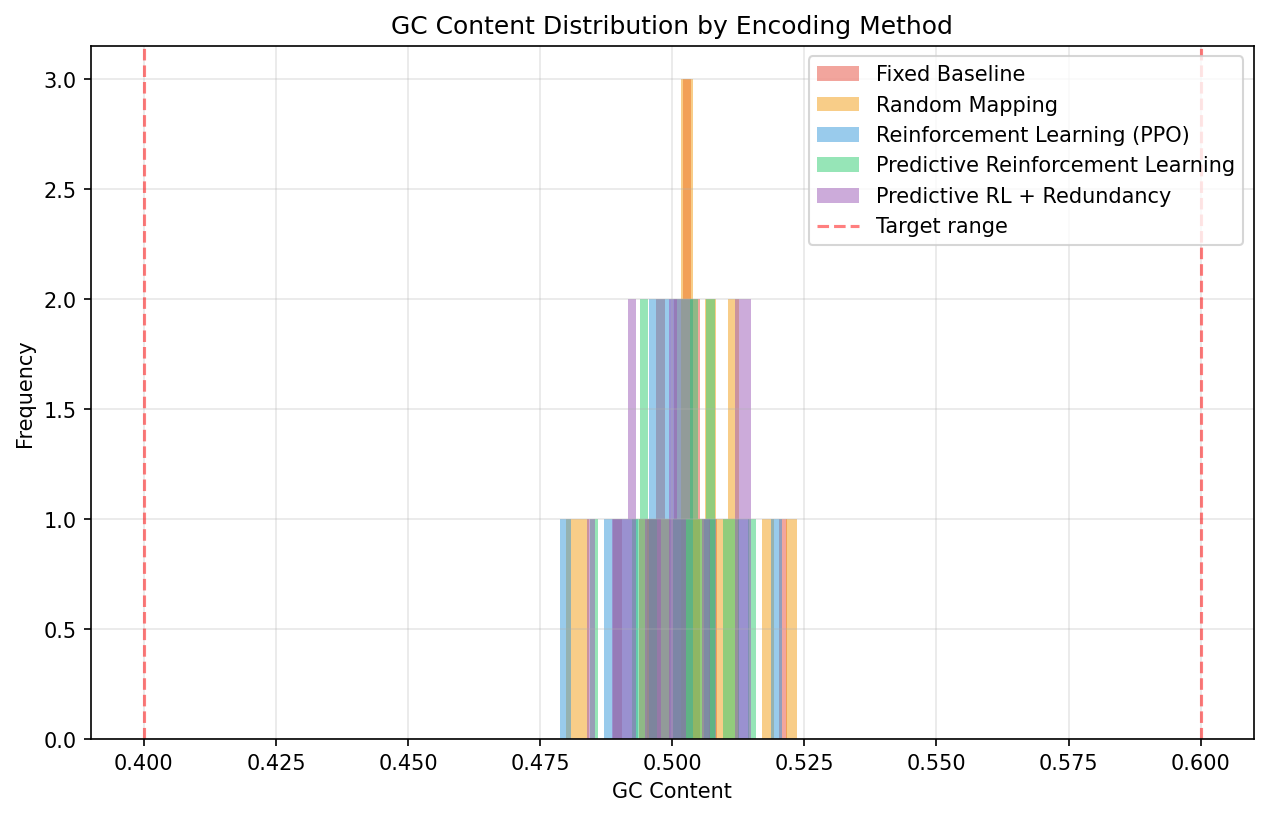
\includegraphics[width=\columnwidth]{figures_for_paper/fig7_gc_content_distribution.png}
\caption{GC~content distribution by method.  RL-based methods cluster more
tightly around the target of 0.50.}
\label{fig:gc_distribution}
\end{figure}

\subsection{Statistical Significance}\label{sec:significance}

Table~\ref{tab:pvalues} reports $t$-statistics and $p$-values from
independent two-sample $t$-tests at each length.

\begin{table}[htbp]
\centering
\caption{Statistical Comparisons ($t$ / $p$, 7~seeds).
$^{*}$~$p<0.05$.}
\label{tab:pvalues}
\renewcommand{\arraystretch}{1.15}
\footnotesize
\begin{tabular}{@{}lccc@{}}
\toprule
\textbf{Comparison} & \textbf{64~nt} & \textbf{128~nt} & \textbf{256~nt} \\
\midrule
Pred.\ RL vs.\ Base & 0.62\,/\,0.57 & 0.96\,/\,0.39 & $-$0.52\,/\,0.63 \\
Pred.\ RL vs.\ RL   & 2.59\,/\,0.061 & 4.97\,/\,\textbf{0.008}$^{*}$ & $-$0.23\,/\,0.83 \\
RL vs.\ Baseline     & $-$1.90\,/\,0.13 & $-$7.07\,/\,\textbf{0.002}$^{*}$ & $-$0.17\,/\,0.87 \\
\midrule
& \textbf{512~nt} & \textbf{1024~nt} & \\
\midrule
Pred.\ RL vs.\ Base & 0.45\,/\,0.67 & 0.03\,/\,0.98 & \\
Pred.\ RL vs.\ RL   & 0.39\,/\,0.71 & $-$0.59\,/\,0.59 & \\
RL vs.\ Baseline     & $-$0.01\,/\,0.99 & 0.53\,/\,0.62 & \\
\bottomrule
\end{tabular}
\end{table}

Two comparisons reach significance.  At 128~nt the predictive agent
outperforms the predictor-free agent ($p = 0.008$, $t = 4.97$), confirming
a genuine contribution of error-aware reward shaping.  The same predictor-free
agent falls significantly \emph{below} baseline at that length ($p = 0.002$,
$t = -7.07$), revealing that without the corrective signal the RL agent
over-optimises for GC~balance and homopolymer avoidance at the cost of decode
accuracy.

At 64~nt the predictive-vs-RL comparison approaches significance
($p = 0.061$).  At longer lengths (256--1024~nt) no pair-wise differences
are significant, consistent with the convergence of single-copy methods
discussed above.

\subsection{Multi-Copy Redundancy Scaling}

Table~\ref{tab:redundancy} and Fig.~\ref{fig:redundancy} show how decode
accuracy scales when the number of stored copies is increased from 1 to~10.

\begin{table}[htbp]
\centering
\caption{Decode Accuracy (\%) vs.\ Number of Copies
(mean~$\pm$~std, Predictive~RL)}
\label{tab:redundancy}
\renewcommand{\arraystretch}{1.1}
\footnotesize
\begin{tabular}{@{}cccccc@{}}
\toprule
\textbf{$N$} & \textbf{64} & \textbf{128} & \textbf{256} & \textbf{512} & \textbf{1024} \\
\midrule
1  & 76.29{\scriptsize$\pm$1.53} & 70.72{\scriptsize$\pm$1.10} & 62.37{\scriptsize$\pm$1.44} & 59.85{\scriptsize$\pm$0.46} & 57.16{\scriptsize$\pm$0.59} \\
3  & 81.96{\scriptsize$\pm$0.94} & 72.99{\scriptsize$\pm$1.23} & 67.49{\scriptsize$\pm$0.99} & 61.70{\scriptsize$\pm$0.47} & 58.98{\scriptsize$\pm$0.30} \\
5  & 85.03{\scriptsize$\pm$1.12} & 76.20{\scriptsize$\pm$1.10} & 69.69{\scriptsize$\pm$1.14} & 64.93{\scriptsize$\pm$0.09} & 60.55{\scriptsize$\pm$0.19} \\
7  & 86.16{\scriptsize$\pm$0.41} & 78.17{\scriptsize$\pm$1.08} & 71.82{\scriptsize$\pm$1.02} & 66.36{\scriptsize$\pm$0.37} & 61.80{\scriptsize$\pm$0.24} \\
10 & \textbf{88.72}{\scriptsize$\pm$0.20} & \textbf{79.39}{\scriptsize$\pm$0.71} & \textbf{73.61}{\scriptsize$\pm$0.21} & \textbf{67.27}{\scriptsize$\pm$0.24} & \textbf{62.96}{\scriptsize$\pm$0.18} \\
\bottomrule
\end{tabular}
\end{table}

\begin{figure}[!t]
\centering
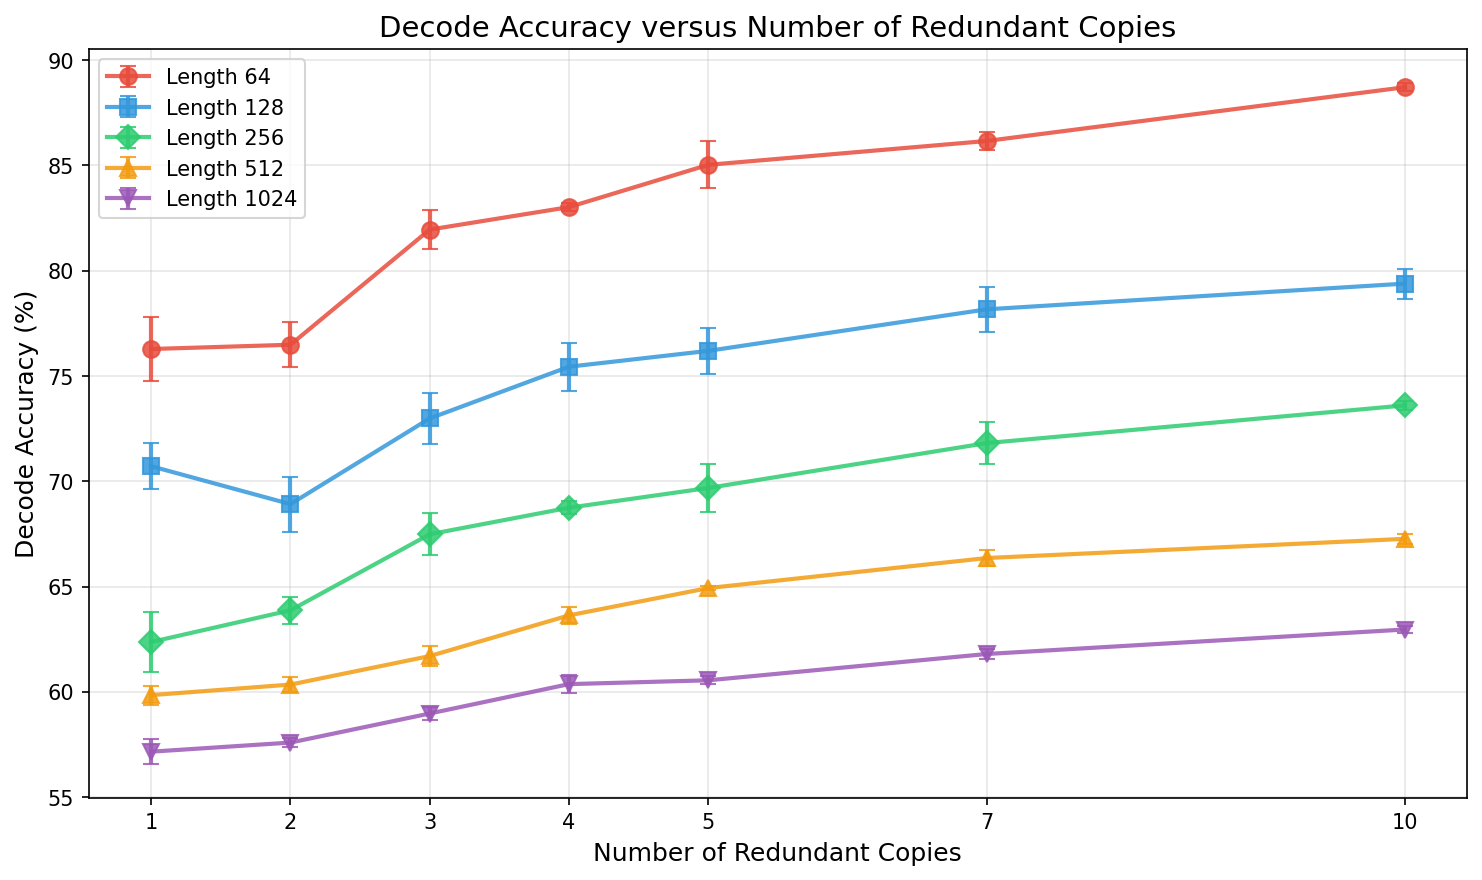
\includegraphics[width=\columnwidth]{figures_for_paper/fig11_redundancy_scaling.png}
\caption{Decode accuracy versus number of copies at five lengths.  Error bars
show $\pm1$~std over seven seeds.  Improvement is monotonic at every length,
with diminishing marginal returns.}
\label{fig:redundancy}
\end{figure}

Ten copies push accuracy to 88.72\%$\pm$0.20\% at 64~nt---a 12.43~pp gain
over a single copy.  The scaling is monotonic and consistent across all five
lengths.  Even at 1024~nt, where single-copy accuracy is only 57.16\%,
ten-copy voting lifts it to 62.96\% ($+5.80$~pp).  The improvement exhibits
diminishing returns: the jump from 1 to 3~copies contributes roughly half
the total 1-to-10 gain at 64~nt, consistent with the theoretical behaviour
of majority voting under independent errors.


% ══════════════════════════════════════════════════════════════
%  XII.  ABLATION STUDY
% ══════════════════════════════════════════════════════════════
\section{Ablation Study}

To isolate individual reward components, additional agent variants were
trained with specific weights set to zero.  Table~\ref{tab:ablation} and
Fig.~\ref{fig:ablation} summarise the results.

\begin{table}[htbp]
\centering
\caption{Ablation: Error Rate by Condition and Length
(mean~$\pm$~std, 7~seeds). Bold marks the lowest per column.}
\label{tab:ablation}
\renewcommand{\arraystretch}{1.1}
\footnotesize
\begin{tabular}{@{}lccccc@{}}
\toprule
\textbf{Condition} & \textbf{64} & \textbf{128} & \textbf{256} & \textbf{512} & \textbf{1024} \\
\midrule
Baseline    & .340{\scriptsize$\pm$.015} & \textbf{.425}{\scriptsize$\pm$.010} & \textbf{.517}{\scriptsize$\pm$.007} & .592{\scriptsize$\pm$.006} & .627{\scriptsize$\pm$.005} \\
Full RL     & .358{\scriptsize$\pm$.017} & .467{\scriptsize$\pm$.011} & .530{\scriptsize$\pm$.006} & \textbf{.574}{\scriptsize$\pm$.009} & .618{\scriptsize$\pm$.007} \\
Pred.\ RL   & .342{\scriptsize$\pm$.035} & .458{\scriptsize$\pm$.004} & .525{\scriptsize$\pm$.013} & .578{\scriptsize$\pm$.009} & .627{\scriptsize$\pm$.004} \\
w/o GC      & \textbf{.315}{\scriptsize$\pm$.029} & .431{\scriptsize$\pm$.012} & .531{\scriptsize$\pm$.006} & .584{\scriptsize$\pm$.013} & .638{\scriptsize$\pm$.007} \\
w/o Homo    & .333{\scriptsize$\pm$.012} & .455{\scriptsize$\pm$.012} & .533{\scriptsize$\pm$.004} & .584{\scriptsize$\pm$.010} & \textbf{.628}{\scriptsize$\pm$.002} \\
\bottomrule
\end{tabular}
\end{table}

\begin{figure}[!t]
\centering
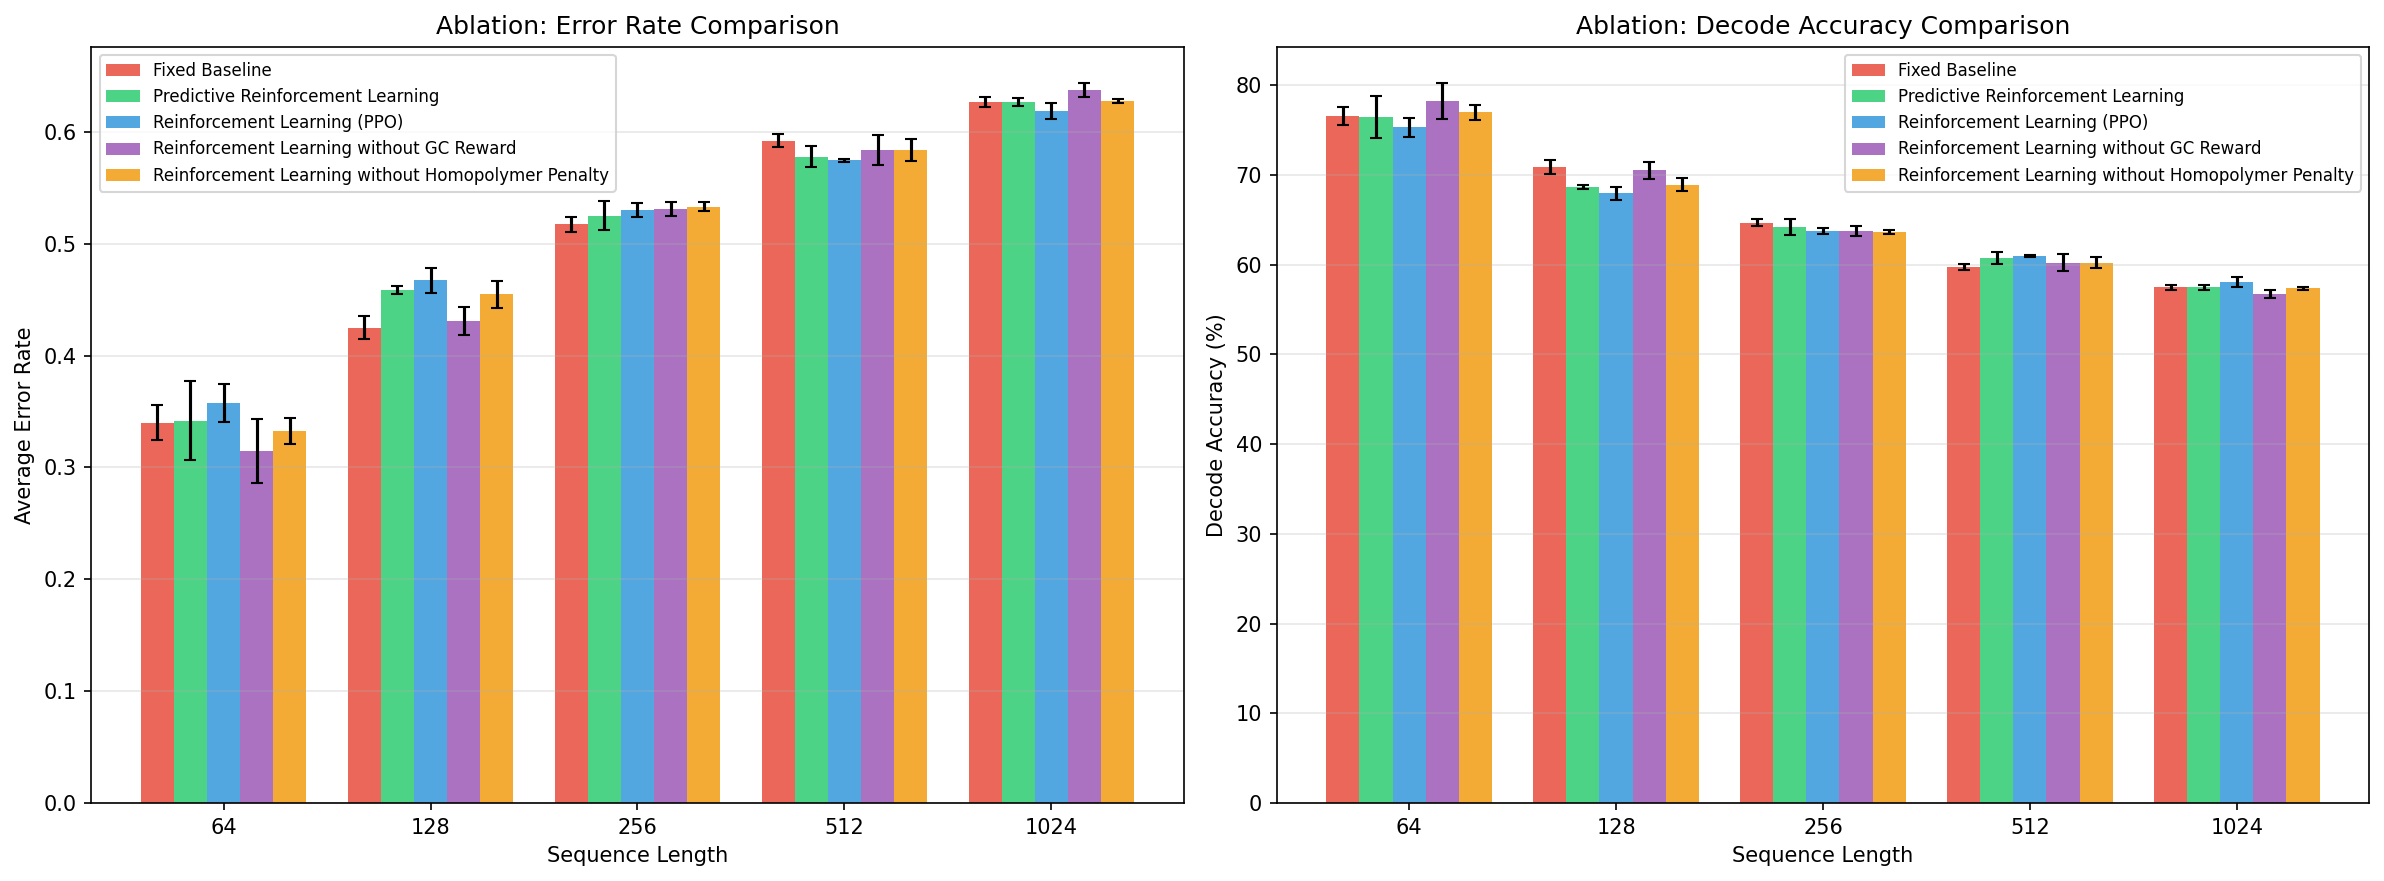
\includegraphics[width=\columnwidth]{figures_for_paper/fig9_ablation_study_comparison.png}
\caption{Ablation study: error rate across five conditions and five lengths.}
\label{fig:ablation}
\end{figure}

Three patterns emerge.  First, dropping the GC~bonus yields the lowest error
rate at 64~nt (0.315), suggesting that GC~pressure can conflict with
error-rate minimisation---though sequences produced without GC~guidance may be
harder to synthesise in practice.  Second, dropping the homopolymer penalty
helps at 128~nt (0.455 vs.\ 0.467 for the full agent) but not at other
lengths.  Third, the full agent achieves the lowest learned-method error rate
at 512~nt (0.574), showing that the complete reward can outperform any single
ablation in some regimes.

These results confirm that the optimal reward balance is length-dependent.
The multi-objective formulation in Eq.~(\ref{eq:reward}) trades decode
accuracy against biophysical quality, and the ablation study quantifies how
that trade-off shifts with sequence length.


% ══════════════════════════════════════════════════════════════
%  XIII.  DISCUSSION
% ══════════════════════════════════════════════════════════════
\section{Discussion}

\subsection{Redundancy as the Primary Driver}

The single most effective mechanism in the pipeline is multi-copy consensus
voting.  Three copies raise accuracy by 5.40~pp at 64~nt relative to a single
copy, and scaling to ten copies adds 12.43~pp.  The gain is monotonic across
every tested length, with diminishing marginal returns that follow the
theoretical expectation for majority voting under independent errors: each
additional copy adds less than its predecessor because the remaining
errors are increasingly correlated across copies.

\subsection{Why the Error Predictor Matters}

Without the predictor, the PPO agent drifts toward policies that score well on
GC~balance and homopolymer avoidance---secondary objectives in the
reward---while inadvertently increasing bit error rate.  This is most visible
at 128~nt, where the predictor-free agent falls significantly below the fixed
baseline ($p = 0.002$).  The predictor injects a direct estimate of sequencing
risk into the reward, counteracting this drift and recovering decode accuracy.
The result is a significant improvement of the predictive agent over the
predictor-free agent at the same length ($p = 0.008$).

At shorter sequences (64~nt) the effect approaches significance
($p = 0.061$).  At longer lengths (256--1024~nt) the 96-action space provides
diminishing leverage, and all single-copy methods converge.

\subsection{Sequence-Length Dependence}

Performance gaps between methods shrink with increasing length.  At 64~nt
the predictive agent enjoys a 0.58~pp edge over baseline; at 1024~nt the
two are essentially tied (57.46\% vs.\ 57.47\%).  This is expected: the
96~composite actions amount to a global choice of mapping, and a single global
choice has less influence over a 1024-position sequence than over a
64-position one.  Per-position or sliding-window encodings, explored in future
work, may address this limitation.

\subsection{Generalisation}

The overfitting check (Table~\ref{tab:overfit}) shows train--test gaps below
1.24~pp everywhere, with four of five lengths exhibiting slightly higher test
accuracy.  This is consistent with the relatively small model capacity
($2 \times 64$ hidden units) and the use of dropout ($p = 0.1$), which
together limit the risk of memorising training distributions.


% ══════════════════════════════════════════════════════════════
%  XIV.  LIMITATIONS
% ══════════════════════════════════════════════════════════════
\section{Limitations}

\begin{enumerate}
    \item \textbf{Simulated error channel.}  All evaluations rely on a
    controlled simulation with fixed base rates (2\% substitution, 1\%
    insertion, 1\% deletion) and heuristic context modulation.  Real
    sequencing platforms introduce position-dependent, technology-specific
    error patterns not captured here.

    \item \textbf{Constrained action space.}  The 96~composite mappings
    represent a relatively small action space.  More flexible schemes
    permitting per-position decisions could yield larger improvements.

    \item \textbf{No algebraic error correction.}  The evaluation omits
    Reed--Solomon or fountain codes~\cite{erlich2017}, which are standard in
    practical DNA storage pipelines.  Whether learned encodings interact
    synergistically with such codes remains untested.

    \item \textbf{Synthetic data only.}  Training and evaluation used
    synthetically generated binary data with controlled distributions.
    Performance on real-world payloads (compressed files, images, genomic
    data) has not been assessed.

    \item \textbf{Network capacity.}  The $2 \times 64$ Tanh backbone limits
    representational power.  Larger or attention-based architectures may learn
    more effective policies.
\end{enumerate}


% ══════════════════════════════════════════════════════════════
%  XV.  FUTURE WORK
% ══════════════════════════════════════════════════════════════
\section{Future Work}

\begin{enumerate}
    \item \textbf{Wet-lab validation.}  Testing the learned encodings against
    empirical error profiles from Illumina, Oxford Nanopore, or PacBio
    platforms would establish practical utility.

    \item \textbf{Richer error predictors.}  Convolutional or recurrent
    architectures may improve error estimation at longer lengths where local
    context effects accumulate.

    \item \textbf{Integration with error-correcting codes.}  Studying
    interaction effects between learned mappings and Reed--Solomon or fountain
    codes could reveal synergies.

    \item \textbf{Per-position encoding.}  Expanding the action space to
    per-dibit or per-position decisions may increase adaptability, especially
    for longer sequences.

    \item \textbf{Adaptive reward weighting.}  The ablation study shows that
    optimal component weights vary with length.  Meta-learning or multi-task
    reward design may improve robustness.

    \item \textbf{Oligo chunking.}  Segmenting long data streams into
    short addressed blocks (64--128~nt), encoding each independently, and
    reassembling upon retrieval---following practical
    pipelines~\cite{organick2018}---would scale the method to arbitrary data
    sizes while preserving short-length accuracy.
\end{enumerate}


% ══════════════════════════════════════════════════════════════
%  XVI.  CONCLUSION
% ══════════════════════════════════════════════════════════════
\section{Conclusion}

We have presented a three-layer system for adaptive DNA data encoding that
pairs a PPO-based agent with a neural error predictor and multi-copy consensus
voting.  Evaluation over seven independent seeds and five sequence lengths
yields the following principal results.

First, consensus voting is the dominant contributor to accuracy.  Three copies
raise decode accuracy from 76.56\% to 81.96\% at 64~nt ($+5.40$~pp); ten
copies reach 88.72\%$\pm$0.20\%, a 12.43~pp improvement that scales
monotonically across all tested lengths.

Second, the error predictor is a necessary component.  At 128~nt the
predictor-free agent falls significantly below baseline ($p = 0.002$), while
the predictive agent significantly exceeds the predictor-free agent
($p = 0.008$), confirming that error-aware reward shaping prevents the
policy from trading accuracy for secondary objectives.

Third, the predictive agent matches or exceeds baseline accuracy while
producing sequences with markedly higher biophysical quality (stability
scores of 0.902--0.945 vs.\ 0.857--0.898).

Fourth, the ablation study shows that the optimal reward composition is
length-dependent, and the overfitting check confirms train--test gaps below
1.24~pp at every length.

Taken together, these findings demonstrate that even a modest 96-action
learned encoding, when paired with error-aware reward shaping and multi-copy
voting, can meaningfully improve the reliability of DNA-based data storage.
Validation under real biological sequencing conditions remains essential
before practical deployment.


% ══════════════════════════════════════════════════════════════
%  REFERENCES
% ══════════════════════════════════════════════════════════════
\begin{thebibliography}{00}

\bibitem{reinsel2018}
D.~Reinsel, J.~Gantz, and J.~Rydning, ``The digitization of the world---from
edge to core,'' International Data Corporation (IDC), White Paper, Nov.~2018.

\bibitem{church2012}
G.~M.~Church, Y.~Gao, and S.~Kosuri, ``Next-generation digital information
storage in DNA,'' \textit{Science}, vol.~337, no.~6102, p.~1628, Sep.~2012.

\bibitem{grass2015}
R.~N.~Grass, R.~Heckel, M.~Puddu, D.~Paunescu, and W.~J.~Stark, ``Robust
chemical preservation of digital information on DNA in silica with
error-correcting codes,'' \textit{Angewandte Chemie International Edition},
vol.~54, no.~8, pp.~2552--2555, Jan.~2015.

\bibitem{goldman2013}
N.~Goldman \textit{et al.}, ``Towards practical, high-capacity,
low-maintenance information storage in synthesized DNA,'' \textit{Nature},
vol.~494, no.~7435, pp.~77--80, Jan.~2013.

\bibitem{erlich2017}
Y.~Erlich and D.~Zielinski, ``DNA Fountain enables a robust and efficient
storage architecture,'' \textit{Science}, vol.~355, no.~6328, pp.~950--954,
Mar.~2017.

\bibitem{organick2018}
L.~Organick \textit{et al.}, ``Random access in large-scale DNA data
storage,'' \textit{Nature Biotechnology}, vol.~36, no.~3, pp.~242--248,
Feb.~2018.

\bibitem{ross2013}
M.~G.~Ross \textit{et al.}, ``Characterizing and measuring bias in sequence
data,'' \textit{Genome Biology}, vol.~14, no.~5, R51, May~2013.

\bibitem{heckel2019}
R.~Heckel, G.~Mikutis, and R.~N.~Grass, ``A characterization of the DNA data
storage channel,'' \textit{Scientific Reports}, vol.~9, no.~1, p.~9663,
Jul.~2019.

\bibitem{schirmer2015}
M.~Schirmer, U.~Z.~Ijaz, R.~D'Amore, N.~Hall, W.~T.~Sloan, and C.~Quince,
``Insight into biases and sequencing errors for amplicon sequencing with the
Illumina MiSeq platform,'' \textit{Nucleic Acids Research}, vol.~43, no.~6,
e37, Mar.~2015.

\bibitem{sutton2018}
R.~S.~Sutton and A.~G.~Barto, \textit{Reinforcement Learning: An
Introduction}, 2nd~ed.\hskip 1em Cambridge, MA, USA: MIT Press, 2018.

\bibitem{mazyavkina2021}
N.~Mazyavkina, S.~Sviridov, S.~Ivanov, and E.~Burnaev, ``Reinforcement
learning for combinatorial optimization: A survey,'' \textit{Computers \&
Operations Research}, vol.~134, p.~105400, Oct.~2021.

\bibitem{angermueller2020}
C.~Angermueller, D.~Dohan, D.~Belanger, R.~Deshpande, K.~Murphy, and
L.~Colwell, ``Model-based reinforcement learning for biological sequence
design,'' in \textit{Proc.\ Int.\ Conf.\ Learning Representations (ICLR)},
Apr.~2020.

\bibitem{schulman2017}
J.~Schulman, F.~Wolski, P.~Dhariwal, A.~Radford, and O.~Klimov, ``Proximal
Policy Optimization Algorithms,'' \textit{arXiv preprint arXiv:1707.06347},
Jul.~2017.

\end{thebibliography}

\end{document}
